% mn2esample.tex
%
% v2.1 released 22nd May 2002 (G. Hutton)
%
% The mnsample.tex file has been amended to highlight
% the proper use of LaTeX2e code with the class file
% and using natbib cross-referencing. These changes
% do not reflect the original paper by A. V. Raveendran.
%
% Previous versions of this sample document were
% compatible with the LaTeX 2.09 style file mn.sty
% v1.2 released 5th September 1994 (M. Reed)
% v1.1 released 18th July 1994
% v1.0 released 28th January 1994

\documentclass[useAMS,usenatbib]{mn2e}
\usepackage{graphics}
\usepackage{graphicx}
\usepackage{epsfig}
\usepackage{amsmath}

\voffset-1.25cm

% If your system does not have the AMS fonts version 2.0 installed, then
% remove the useAMS option.
%
% useAMS allows you to obtain upright Greek characters.
% e.g. \umu, \upi etc.  See the section on "Upright Greek characters" in
% this guide for further information.
%
% If you are using AMS 2.0 fonts, bold math letters/symbols are available
% at a larger range of sizes for NFSS release 1 and 2 (using \boldmath or
% preferably \bmath).
%
% The usenatbib command allows the use of Patrick Daly's natbib.sty for
% cross-referencing.
%
% If you wish to typeset the paper in Times font (if you do not have the
% PostScript Type 1 Computer Modern fonts you will need to do this to get
% smoother fonts in a PDF file) then uncomment the next line
% \usepackage{Times}

%%%%% AUTHORS - PLACE YOUR OWN MACROS HERE %%%%%

%\newcommand{\Mvir}{$\rm M_{\rm vir}$}
%\newcommand{\Rvir}{$\rm R_{\rm vir}$}
%\newcommand{\cvir}{$\rm c_{\rm vir}$}
%\newcommand{\Ms}{$\rm M_{\rm s}$}
%\newcommand{\rs}{$\rm r_{\rm s}$}

%\newcommand{\hMpc}{$h^{-1}\rm{Mpc}$}
%\newcommand{\hMsun}{$\rm {M_{\odot}h^{-1}}$}

\newcommand{\Rq}{$\rm R_{1/4} $}
\newcommand{\etal}{et al.~}
\newcommand{\rhocrit}{\rho_c}
\newcommand{\rhorms}{\rho_{\rm rms}}
\newcommand{\xoff}{x_{\rm off}}
\newcommand{\cvir}{c_{\rm vir}}
\newcommand{\Rvir}{R_{\rm vir}}
\newcommand{\Mvir}{M_{\rm vir}}
\newcommand{\rs}{r_{\rm s}}
\newcommand{\Jvir}{J_{\rm vir}}
\newcommand{\Vvir}{V_{\rm vir}}
\newcommand{\Nvir}{N_{\rm vir}}
\newcommand{\Ms}{M_{\rm s}}

\def \kms {\ifmmode  \,\rm km\,s^{-1} \else $\,\rm km\,s^{-1}  $ \fi }
\def \kpc {\ifmmode  {\rm kpc}  \else ${\rm  kpc}$ \fi  }  
\def \Msun {\ifmmode M_{\odot} \else $M_{\odot}$ \fi} 
\def \hMsun {\ifmmode h^{-1}\,\rm M_{\odot} \else $h^{-1}\,\rm M_{\odot}$ \fi}
\def \hMpc {\ifmmode h^{-1}\,\rm Mpc \else $h^{-1}\,\rm Mpc$ \fi}
\def \hkpc {\ifmmode h^{-1}\,\rm kpc \else $h^{-1}\,\rm kpc$ \fi}
\def \hLsun {\ifmmode h^{-1}\,\rm L_{\odot} \else $h^{-1}\,\rm L_{\odot}$ \fi}

\newcommand{\mnras}{MNRAS}
\newcommand{\apj}{ApJ}
\newcommand{\apjl}{ApJ}
\newcommand{\apjs}{ApJS}
\newcommand{\aj}{AJ}
\newcommand{\aap}{A\&A}
\newcommand{\nat}{Nature}


%%%%%%%%%%%%%%%%%%%%%%%%%%%%%%%%%%%%%%%%%%%%%%%%%%%%%%%%%%%%%%%%
%%%%%%%%%%%%%%%%%%%%%%%%%%%%%%%%%%%%%%%%%%%%%%%%%%%%%%%%%%%%%%%%

\title[How abundant are the Local Group galaxies?]
{How abundant are the Local Group galaxies?}
\author[mengano, et al.]
{fulano, perano mengano. Disc survival collaboration UdeA-AIP$^{1}$$^{2}$\\
$^{1}$ Leibniz-Institut F\"{u}r Astrophysik Potsdam, An der Sternwarte 16, 14482
Potsdam, Germany.\\
$^{2}$ Instituto de Fisica, Universidad de Antioquia, Medellin, Colombia.
}
\begin{document}

\date{Accepted XXXX December XX. Received XXXX December XX; in original form
  2009 June 27}

\pagerange{\pageref{firstpage}--\pageref{lastpage}} \pubyear{2002}

\maketitle

\label{firstpage}

\begin{abstract}
  
We present a series of models that follow the evolution of the two
dominant galaxies in the Local Group: the Milky Way (MW) and M31. We
use semi-analytic techniques coupled to three N-body constrained
cosmological simulations. Each simulated volume contains a pair of
halos with environmental conditions similar to the observed for the
LG. The models are computed using the public available code
Galacticus. The main objective is to study the conditions to get the
best possible agreement in three baryonic properties for the MW and
M31: the stellar mass, gaseous mass and disc-to-bulge mass ratio. Each
physical model varies the parameters controlling the star formation
efficiency and supernovae feedback. The models are run on a general
sample of dark halos with a mass range of $7\times10^{11}\hMsun<M_{\rm
  h}<7\times 10^{12}\hMsun$. For the model that best reproduce the
global properties of galaxies in this halo mass range, we find that
the most probable values for the baryonic properties are $M_{\star}=$,
$M_{\rm gas}=$ and $f_{D/B}=$. The three LG in the constrained
simulation have values $M_{\star}=$, $M_{\rm gas}=$ and $f_{D/B}=$.

\end{abstract}

\begin{keywords}
galaxies: haloes, groups -- cosmology: dark matter, observations
\end{keywords}



%%%%%%%%%%%%%%%%%%%%%%%%%%%%%%%%%%%%%%%%%%%%%%%%%%%%%%%%%%%%%%%%%%%%%%
%%%%%%%%%%%%%%%%%%%%%%%%%%%%%%%%%%%%%%%%%%%%%%%%%%%%%%%%%%%%%%%%%%%%%%


\section{Introduction}

cosmological scenario
the local group
the problem of locating the LG in the universe

The questions we want to address in this paper is: How common is the
local group of galaxies in the cosmological context? what is the
probability of generate a local group in the universe? under which
physical conditions do we reproduce the properties of the galaxies in
the Local Group?



%%%%%%%%%%%%%%%%%%%%%%%%%%%%%%%%%%%%%%%%%%%%%%%%%%%%%%%%%%%%%%%%%%%%%
%%%%%%%%%%%%%%%%%%%%%%%%%%%%%%%%%%%%%%%%%%%%%%%%%%%%%%%%%%%%%%%%%%%%%


\section{Methods} 
\label{sec:method}

\subsection{N-body simulations}
\label{sec:simul}

In this work we study the evolution of galaxies in the Local Universe
through the use of semi-analytic models of galaxy formation. To
properly constrain the study to the Local Group it is required to use
then constrained simulations of the Local Universe. A constrained
simulation is a standard N-body simulation of the formation of
structure in which observational constraints have been imposed on the
initial conditions in order to reproduce the large scale environment
of the local Universe. The simulations used in this work have been
extensively discussed in previous works, we refer the reader seeking
for a detailed description of the procedures and details of the
simulations to these papers (Martinez-Vaquero \etal 2009, Gottl\"{o}ber
\etal 2010, Forero-Romero \etal 2011, Doumler \etal 2012). Here we
will focus only on the details of the simulations that are relevant
for the sake of interest of this paper.

The constrained simulations used in this work are part of a suite of
cosmological simulations part of the CLUES project (Constrained
Simulations of the Local Universe, Gottl\"{o}ber \etal 2010). The
observational constraints impose conditions on the large scale
structure of the local Universe on scales above a few mega parsec,
however the small scales keep unconstrained and behave basically
randomly. In order to overcome this problem, and to obtain a
realisation that matches as close as possible not only the large scale
environment but also the environment of the Local Group, many
realisations are required of the same piece of the Universe with the
same constraints. From this set of realisations a few have been
selected to be potential candidates in which not only the large scale
environment but also the small scale environment have been
satisfactorily reproduced.

The criteria used to identify fiducial a Local Group realisation among
this set of 200 are (see Forero-Romero \etal 2011)

\begin{itemize}

\item The distance between neighbour haloes is smaller than 0.7\hMpc
  (Ribas \etal 2005)

\item The relative radial velocity of the two haloes is negative.

\item There must be no objects more massive than either of the LG host
  haloes within a radius of 2\hMpc from each other (Tikhonov \& Klypin
  2009)

\item There must be no a halo of mass $>5.0\times10^{13}\hMsun$ within
  a radius of 5\hMpc with respect to each halo centre (Karachentsev
  \etal 2004)

\end{itemize}

From a set of 200 low resolution realisations, only three were found
to meet the aforementioned conditions to host a potential local
group. These three simulations where resimulated at higher resolution
with a box size of 64 \hMpc and sampled with $1024^3$ particles giving
a particle mass of $1.89\times10^7$ \hMsun. The candidates to Milky
Way (MW) and Andromeda galaxy (M31) in these simulations are resolved
with more than 50000 particles. Simulations were performed with the
cosmological Tree-PM code Gadget-2 (Springel 2005) and the starting
redshift of the simulations was 50.

The use of the constrained simulations provide us with the unique
opportunity to model the large and small scale environment of the
Local Group, and pick candidate objects to host the M31 and M31
galaxies. Simultaneously, the realisation of simulations of dark
matter only provide us with the opportunity to simulate a large sample
of galaxies. For each of the three simulations we have around 10000
haloes identified with more than 200 particles, and around 9000 haloes
in the mass range $10^{11}\Msun$ to $10^{13}\Msun$. In general,
combining the three data sets we have a total of ~27000 haloes in the
mass range of $10^{11}\Msun$ to $10^{13}\Msun$, which provide us with
a large statistical sample of MW type haloes.

In our simulations halos are identified using a FoF method with a
linking lenght of $b=0.17$ times the mean interpartilce distance and a
at least 20 member particles. Haloes are identified in 80 snapshots
roughly equally spaced in time between $z=0$ and $z=7$. The merger
tree construction is based on the comparison of the particles in FOF
groups in two consecutive snapshots. Starting at $z=0$ for every FOF
group in the catalog, G0, we find all the FOF groups in the previous
snapshots that share at least thirteen particles with G0 and label
them as tentative progenitors. Then, for each tentative progenitor, we
find all the descendants sharing at least thirteen particles. Since
the smallest FOF groups contain 20 particles at least 2/3 of the
particles must be identified in tentative progenitors or
descendants. Only the tentative progenitors that have as a main
descendant the group G0 are labeled as confirmed progenitors at that
level. We iterate this procedure for each confirmed progenitor, until
the last available snapshot at high redshift. By construction, each
halo in the tree can have only one descendant, but many progenitors

The merger histories used in this work have been studied in detail in
Forero-Romero \etal 2011, we recommend the reader to take a look on
this paper to find more details on the tree construction and the
properties of the merger histories we use in this work.

\subsection{Semi-analytic Modelling} 
\label{sec:sam}

Since the simulations we use are dark matter only, galaxy formation
has to be modelled as an external process happening inside dark matter
haloes. One of the advantages of using this semi-analytic approach is
the opportunity to explore the parameter space and to find the
parameter set that best reproduce the observed structure of the Local
Group galaxies.

Instead of developing our own semi-analytic code of galaxy formation,
we opted for the alternative to use a publicly available one. The code
we used in this work is GALACTICUS, a semi-analytic code developed by
Andrew Benson (Benson 2012). GALACTICUS implements several physical
processes and implements different approaches for each
process. Instead of exploring the many different possibilities of the
code, we keep close to the ``default model'' of the code and used
standard recipes to model the different physical processes as
described in (Benson 2012).

In our simulations we have included many different physical processes:
Radiative cooling, star formation, energy feedback processes, chemical
enrichment, mass transfer between components, galaxy mergers, galactic
structure, etc. No AGN feedback has been considered since we focus on
a low halo mass regime where AGN effect should not play an important
role.

Each physical process is controlled by one or more parameters. From
that large set of physical processes we focus our attention on a few
ones, under the assumption that these processes are the ones that most
affect the final state of the galaxies forming inside the haloes of
the simulation. For these models we have decided to vary
systematically its parameters in order to explore the parameter space
associated with the probability of having Local Group like galaxies
(LG-like galaxies). After exploring the parameter space, we choose to
study in detail the changes in the population of galaxies under
variations of the physical parameters controlling the star formation
time scale ($\epsilon_{\star}$, $\alpha_\star$), supernovae feedback
($\alpha_{\rm out}$) and the mass ratio defining the major/minor
merger threshold.


\subsubsection{Galaxy mass growth}

One would expect that the accretion of cold gas in a dark matter halo
depends on the mass growth rate of the halo, but also on the available
gas mass, the mass of the halo itself and the thermodynamical
conditions of the gas. In GALACTICUS we use the {\em simple} method to
model the accretion of cold gas like

\begin{equation}
 \dot{M}_{\rm accr}=
 \begin{cases}
   (\Omega_b/\Omega_M)\dot{M}_{{\rm halo}} & \mbox{if } V_{\rm vir}>V_{\rm reioniz}\\
                                        & \mbox{or } z>z_{\rm reioniz}\\
   0                                    & \mbox{otherwise }
\end{cases}
\end{equation}


where $\Omega_b/\Omega_M$ is the cosmic baryon fraction that basically
controls the amount of available baryons and $V_{\rm reioniz}$ and
$z_{\rm reioniz}$ are the free parameters that control the accretion
of cold gas accretion. If a halo has a low virial velocity $V_{\rm
  vir}$ (lower than the threshold $V_{\rm reioniz}$) it is not massive
enough to accrete and keep the cold gas. Also, if the redshift is
larger than $z_{\rm reioniz}$ the temperature of the gas should be
high enough and no effective cooling should be present.


\subsubsection{Star formation time scale}

We have used the standard Cole \etal 2000 star formation time
scale. It is parametrised by a power law in the halo velocity

\begin{equation}
 \tau_{\star} = \epsilon^{-1}_{\star}\tau_{{\rm dyn}}\left(
 \frac{V}{200{\rm km/s}}\right)^{\alpha_\star}
\end{equation}

with free parameters $\epsilon_{\star}$ and $\alpha_\star$ that
controls the star formation efficiency and the shape on the velocity
(or mass) dependence of the star formation time scale.


\subsubsection{Supernova feedback}

The main energy feedback process of the model is the supernova
feedback. Mass ejection from supernovae is modeled as

\begin{equation}
 \dot{M}_{\rm out}=\left( \frac{V_{\rm out}}{V}
 \right)^{\alpha_{\rm out}}\frac{\dot{E}}{E_{\rm canonical}}, \label{eq:supernovae}
\end{equation}

where $V_{\rm out}$ is a threshold velocity for the galactic
component. The larger the value of $V_{\rm out}$ the stronger the
suppression of the outflow of mass. The second parameter is
$\alpha_{\rm out}$, and as $\alpha_\star$ controls the mass dependence
of the outflow. $V$, $\dot{E}$ and $E_{\rm canonical}$ are not
constants, they are the velocity of the component, the rate of energy
input from the stellar populations and the energy input by a stellar
population normalised to $1 {\rm M}_{\odot}$ after an infinite time.


\subsubsection{Minor/Mayor merger ($\eta$)}

We define a minor merger between a massive halo $M_{Hm}$ and a low
mass halo $M_{Lm}$ if

\begin{equation}
\frac{M_{Lm}}{M_{Hm}} \leq \eta
\end{equation}

where $\eta$ is the threshold that defines the nature of the
merger. In other case the merger will represent a major merger.


\subsubsection{Merger mass flow}

After a minor or major merger the mass of the galaxies must be
redistributed in the remnant. The way the mass is redistributed in the
remnant depends on the characteristics of the merger.

\begin{itemize}

\item
If the merger is a major merger the structure of both galaxies is
destroyed and all mass from both galaxies moves to the spheroid of the
remnant central galaxy.

\item
In the case of a minor merger the mass of the satellite moves to the
component that is indicated by the respective flag {\em goes to},
$M_{{\rm satel.,gas}}\to$, where in our case gas and stars can move
from the satellite to the disk or to the bulge of the central galaxy.

\end{itemize}


\subsubsection{Galaxy structure: Spin and concentration parameter}

The structural properties of the galaxy depend partially on the
structural properties of the dark matter halo. We used the approach
included in GALACTICUS that allows to use the fitting formulae of
Prada \etal 2011 to model the concentration parameter of halos as a
function of mass and redshift. For the spin parameter we assume that
this parameter follows a log-normal distribution with mean
$\mu_{\lambda} = 0.031$ and variance $\sigma_{\lambda} = 0.57$ as
computed from cosmological simulations by Mu\~noz-Cuartas \etal
(2011).


\subsection{Observational samples and definition of our local group}
\label{sec:LGdefine}

We have already shown in section \ref{sec:simul} how do we define the
Local Group galaxy candidates in our simulations. Now we need to
introduce an operational definition for these galaxies from the
observational point of view in order to be able to compare the
observations with our simulations. Clearly, MW and M31 are
characterised by its observational properties. Considering the
quantities we can reliably model using the semi-analytic approach we
define or characterise the LG galaxies according to the observed
values of their disk stellar mass ($M_{d,\star}$), disk mass gas
$M_{d,gas}$, bulge stellar mass $M_{b,\star}$ and maximum circular
velocity $V_{\rm cmax}$.


\begin{table}
\centering
\begin{tabular}{|l|l|l|l|l|}
\hline
\hline
 Property & MW & Ref. & M31 & Ref.\\
\hline
$M_{d,\star}[10^{10}M_{\odot}]$       & $3.3-4.5 $ & $(1)$  & $7-10$      & $(2)$ \\
$M_{d,gas}[10^{10}M_{\odot}]$         & $0.6-0.8$  & $(3)$  & $0.5-0.6$  & $(4)$ \\
$M_{b,\star}[10^{10}M_{\odot}]$       & $0.5-1.2$  & $(3)$  & $1.9-3.3$   & $(2)$ \\
$V_{\rm cmax}[\text{Km/s}]$         & $238$      & $(5)$  & $275\pm 5$  & $(6)$ \\
\hline
\hline
\end{tabular}
\caption{Observational estimations for different properties of the LG,
  where$(1)$\citet{2001ApJ...555..393Z},$(2)$
  \citet{2006MNRAS.366..996G}, $(3)$\citet{2009A&A...505..497Y}, $(4)$
  \citet{2006A&A...453..459N}, $(5)$\citet{2005MNRAS.364..433B},
  $(6)$\citet{2008MNRAS.389.1911S}.}
\label{tab:lg-observations}
\end{table}


{\bf Disk stellar mass}. The principal approach to estimate the
stellar mass in the disk of our galaxy is dynamical modelling. The
work of \cite{Klypin2002} uses a parametric model that does not
distinguish between the cold (gas) component and the stars, their
results for galaxy models that allow for exchange of angular momentum
locate the total baryonic mass of the disk between $5-6\times
10^{10}$\Msun for the MW and $7-9\times 10$\Msun for M31. Later
\cite{Widrow2005} use N-body realisations of self-consistent
equilibrium distributions of the dark matter and stellar components to
address the same problem. Their models with good match to the
observational data have stellar masses of $3.3-4.5\times 10^{10}$\Msun
for the Milky Way and $7-10\times 10^{10}$ for
Andromeda. \citep{Geehan2006} modeled the Andromeda stream using
analytic bulge-disc-halo models for M31, finding the best agreement
for a disk mass of $8.4\times 10^{10}$\Msun. In this work we take
$3.3-4.5\times 10^{10}$\Msun for the Milky Way and $7-10\times
10^{10}$ for M31.

{\bf Bulge stellar mass}. \cite{Klypin2002} constrain the MW bulge
stellar mass to $1-1.2\times 10^{10}$ \Msun while for M31
$1.9-2.4\times 10^{10}$. For the same galaxy \citep{Geehan2006} find a
bulge mass of $3.3\times 10^{10}$\Msun. The MW analytic model of
\citep{Dehnen1998} finds a range of different values with average
$\sim 0.5 10^{10}$\Msun. In this work we pick $0.5-1.2 \times
10^{10}$\Msun for the MW and $1.9-3.3\times 10^{10}$\Msun for M31.

{\bf Disk Gaseous mass}. The abundance of gas in the Milky Way has
been constrained through chemical evolution models. The set of
observational constraints on these models most notably include the gas
and star formation rate (SFR) profiles. The relevant observational
data was compiled in \citep{Boissier99} based on the original work in
\cite{Kulkarni87,Dame93}, with values of $6.0-8.0 \times 10^{9}$\Msun.
An updated implementation of this chemical evolution model by
\citep{Yin09} uses the same observations. In the case of M31 the best
observational constraints come from the observations by \citep{Cram80}
with the integrated mass of neutral gas corrected by \citep{Dame93},
yielding a value of $5.2\times 10^{9}$\Msun, there is a systematic
observational uncertainty of $5\%$ originally quoted in
\citep{Cram80}, but due to opacity effects of the HI \citep{Braun92}
the total value of gas can increase by a $19\%$. Therefore we keep a
value of $5.0-6.0\times 10^{9}$ for the mass of gas in the M31 disk
and $6.0-8.0\times 10^{9}$\Msun for the Milky Way.

Table \ref{tab:lg-observations} summarises the values we used to
define each LG-like galaxy, including error bars, which will be
important for the comparison analysis.

\subsection{Analysis strategy}
\label{sec:strategy}


\begin{table*}
\centering
\begin{tabular}{|l|l|l|l|l|l|l|l|l|}
\hline
\hline
Model  &  $z_{reioniz}$ &  $M_{{\rm satel.,gas}}\to$  & $\eta$ & $P(\lambda)$  &  $\mu_\lambda$
 & $\sigma_\lambda$  & $\alpha_{{\rm disk,outflow}}$ & $\epsilon_{{\rm disk},\star}$ \\
\hline
\hline


%run-v2 & 7.0 &  bulge & 0.3 &Lognormal & 0.03687 & 0.2216 & 2.0 & 0.01 \\
%R1 & 9.0 &  bulge & 0.3 &Bett 2007 & &  & 2.0 & 0.01 \\
R2 & 7.0 &  bulge & 0.3 &Lognormal & 0.031 & 0.57 & 2.0 & 0.01 \\
R3 & 7.0 &  disk & 0.3 &Lognormal  & 0.031  & 0.57 & 2.0 & 0.01 \\
\hline
E1 & 7.0 &  disk & 0.3 &Lognormal  & 0.031 & 0.57 & 2.0 & 0.02 \\
E2 & 7.0 &  disk & 0.3 &Lognormal  & 0.031 & 0.57 & 2.0 & 0.035 \\
E3 & 7.0 &  disk & 0.3 &Lognormal  & 0.031 & 0.57 & 2.0 & 0.05 \\
E4 & 7.0 &  disk & 0.3 &Lognormal  & 0.031 & 0.57 & 2.0 & 0.075 \\
E5 & 7.0 &  disk & 0.3 &Lognormal  & 0.031 & 0.57 & 2.0 & 0.1 \\
\hline
A1 & 7.0 &  disk & 0.3 &Lognormal  & 0.031 & 0.57 & 1.5 & 0.01 \\
A2 & 7.0 &  disk & 0.3 &Lognormal  & 0.031 & 0.57 & 2.5 & 0.01 \\
A3 & 7.0 &  disk & 0.3 &Lognormal  & 0.031 & 0.57 & 3.0 & 0.01 \\
\hline
D1 & 7.0 &  disk & 0.2 &Lognormal  & 0.031 & 0.57 & 2.0 & 0.01 \\
D2 & 7.0 &  disk & 0.4 &Lognormal  & 0.031 & 0.57 & 2.0 & 0.01 \\
\hline
B1 & 7.0 &  bulge & 0.2 &Lognormal & 0.031 & 0.57 & 2.0 & 0.01 \\
B2 & 7.0 &  bulge & 0.4 &Lognormal & 0.031 & 0.57 & 2.0 & 0.01 \\
\hline
\hline
\end{tabular}

\caption{Set of four experiments intended to model the galaxies hosted
  in halos of mass range of $11.0<\log_{10} M_{{\rm
      DM}}<13.0$.}
\label{tab:runs}
\end{table*}


In this work we have two goals. First to determine quantitatively
which is the probability to find a galaxy like MW and M31 in a given
cosmological volume. Second, we want to see which are the values of
the parameters in the model that maximise the probability of finding
such galaxies.

To do so we have already defined quantitatively how a LG-like galaxy
should look like, but we need to quantify how far are our models from
such a definition. From this distance measure we can quantify the
probability of finding LG-like galaxies in the nearby universe.

We define the distance between two galaxies (the defined MW or M31 and
a model galaxy, where by model galaxy we mean one of our 27000
galaxies in our simulations) through the distance measure $d$ defined
as

\begin{equation}
  d = \sqrt{ \sum_{i=1}^N \left( \frac{y_i - m_i}{m_i} \right)^2 }
  \label{eq:distance}
\end{equation}

The distance $d$ indicates the actual distance measure (or difference)
between two points in a space defined by the parameter set $m_i$. The
parameter set $m_i$ is the set of values of quantities associated with
the definition of our LG galaxies, that is, N=4 and $m_i$ refers to
$M_{d,*}$, $V_{\rm cmax}$, $M_{d,gas}$ and $M_{b,*}$ as they appear in
table \ref{tab:lg-observations}. The numbers $y_i$ are the values
associated with those quantities for each model galaxy in our
simulations.

We then compute the value of the distance $d$ from each model galaxy
to the defined galaxies MW and M31 and trough it we quantify the
probability to find such an object in our simulations.


%%%%%%%%%%%%%%%%%%%%%%%%%%%%%%%%%%%%%%%%%%%%%%%%%%%%%%%%%%%%%%%%%%%%%%%
%%%%%%%%%%%%%%%%%%%%%%%%%%%%%%%%%%%%%%%%%%%%%%%%%%%%%%%%%%%%%%%%%%%%%%%
%%%%%%%%%%%%%%%%%%%%%%%%%%%%%%%%%%%%%%%%%%%%%%%%%%%%%%%%%%%%%%%%%%%%%%%

\section{Results}
\label{sec:results}

\begin{figure}
 \includegraphics[scale=0.4,angle=270]{figures/Pb_MW_definition.ps}
\caption{Distribution of $d$ values for the same run (R1) computed
  using four different definitions of the distance measure as
  described in the text.}
\label{fig:Pb_MW_definition}
\end{figure}


Now we present the results of our research. First in section
\ref{sec:Probabilities} we analyse, without considering the
constrained nature of our simulations, which is the fraction of
galaxies similar to our LG galaxies. To do that we use around 27000
central galaxies hosted in the same number of dark matter haloes in
the mass range $10^{11}\hMsun to 10^{13}\hMsun$ and use the distance
measure \ref{eq:distance} to quantify the proximity of the models to
the observations.

Later in section \ref{sec:LGs} we use explicitly the candidates to MW
and M31 from our three realisations and study how variations on the
parameters ($\alpha, \epsilon$) affect their properties, and
specifically, how do these variations produce model galaxies that are
in agreement with the observational constraints.


\subsection{On the fraction of Local Group galaxies}
\label{sec:Probabilities}

First we check that our procedure defines robustly the distance
measure to a LG-like galaxy. One may think that including or removing
one of the quantities $m_i$ from the definition of distance measure
eq. \ref{eq:distance} the distribution of values of $d$ could change
so much that the definition of distance is not robust enough,
affecting drastically our probability estimates and conclusions. To
verify the robustness of the distance measure we compute $d$ removing
cyclically one of the properties used to define it, i.e., using only
$M_{d,*}$, $M_{d,gas}$ and $M_{b,*}$ or using only $M_{d,gas}$,
$M_{b,*}$ and $V_{\rm cmax}$, and so on. Using this check we can see
which is the impact of the specific physical quantity on the distance
measure. Clearly, if variations on the definition leads to
catastrophically different distributions of $d$, it will means that
the defined distance measure is not robust enough and therefore is not
an appropriated measure to quantify the probability of finding LG-like
galaxies.

Figure \ref{fig:Pb_MW_definition} shows the distribution of distances
$d$ computed for the same run (R3 in table \ref{tab:runs}). The
distance measure is computed for the MW galaxy using all the four
galaxy properties, and respectively without the use of the $M_{d,*}$,
$M_{b,*}$, $M_{d,gas}$ and without the use of $V_{\rm cmax}$ for the
determination of the distance $d$.

Note that although in all cases the mode of the distribution places
around the same position $d=1.2$, the shape of the distribution is
almost the same in all cases as well as its width. Note also that if
well the change in the definition does affect the probability
distribution, for example increasing the fraction of galaxies closer
to WM type for definitions in which $M_{d,*}$ is not considered in to
the definition, the differences keep small.

%*discuss the truncation at d=2 The distribution has the same shape
%*independent on the parameters There are differences, more for XXX In
%*general the tail of low d values keep the same form

Note that in general no mass constraint is being used (remember that
we ran this analysis on a population of haloes in the mass range from
$10^{11}$ to $10^{13}$\Msun), so, in principle the scatter we have is
naturally due to the broad halo mass range we are exploring. Reducing
the size of halo mass range clearly would lead to a smaller scatter,
but in no way it would lead to an increase in the frequency at the low
$d$ tail of the distribution.

We conclude that in general our definition of distance measure is
robust enough to make an initial estimate on the distribution of
galaxies in comparison with the LG-like galaxies and that our
conclusions are robust enough.

Once we see that our distance measure is robust enough and that it is
not biased by our choice of physical quantities, we can move to the
analysis of the distribution of the distance measure for the LG-like
galaxies. In Figure \ref{fig:Multiplot_Pb_runalpha} we show the
probability distribution of the distance measure for the set of runs
associated to variations of the parameter $\alpha_{\rm out}$ for both,
MW and M31 galaxy. As it can be seen in the figure, and in agreement
with the previous experiment, for a given galaxy no major variations
on the distribution of the distance measure are observed. The peak
places closer to the same position shown in the previous experiment
but the distribution clearly shows a tail to low $d$ values, which is
more extended for M31 than for MW. In general this means that the
probability of finding objects like M31 is larger than that of finding
MW-like objects. Note also that in general there is not a very strong
variation on $f(d)$ for the different values of $\alpha_{\rm
  out}$. Only a mild increase in the probability of finding the
galaxies with small $d$ values at expenses of the respective decrement
for the distribution at larger $d$ values when $\alpha_{\rm out}$
increases from 1.5 to 3.0. This change is more evident for M31 where
we can see that the frequency of $d$ values (and therefore the
probability) increases from $\sim0.0002$ for $\alpha_{\rm out} = 0.15$
to $\sim0.001$ for $\alpha_{\rm out} = 0.3$. A similar trend may be
seen in the case of MW but since its distribution is more concentrated
is not as noticeable as in the case of M31. This behaviour might imply
that indeed higher values of $\alpha_{\rm out}$ may be needed if one
requires to produce a large sample of LG-like galaxies, or
equivalently, that LG-galaxies may be better characterised by high
values of $\alpha_{\rm out}$.


\begin{figure}
 \includegraphics[scale=0.33,angle=270]{figures/Multiplot_Pb_runalpha.ps}
 \caption{Distribution of $d$ values relative the MW and M31
   galaxies. The different lines correspond to realisations of the
   galaxy catalogue using models in which variations of $\alpha_{\rm
     out}$ where carried out from 0.15 to 0.3 while keeping constant
   the other model parameters. See table \ref{tab:runs} for more
   information about the model parameters.}
 \label{fig:Multiplot_Pb_runalpha}
\end{figure}


A similar behaviour can be seen in Figure
\ref{fig:Multiplot_Pb_runeps} where we show the distribution of $d$
for MW and M31 for the experiment where the parameter under variation
is $\epsilon_{{\rm D},\star}$. For the different values of
$\epsilon_{{\rm D},\star}$ the distribution shows to be more skewed to
low $d$-values than the distribution of the respective experiment for
$\alpha_{\rm out}$, indicating that changes on $\epsilon_{{\rm
    D},\star}$ may influence strongly the probability of finding
galaxies like those in the Local Group. Nevertheless the differences
in the distribution for different values of $\epsilon_{{\rm D},\star}$
are not so big, and in particular low values of $\epsilon_{{\rm
    D},\star}$ may favour the increased fraction of galaxies similar
to these in our defined Local Group.


\begin{figure}
 \includegraphics[scale=0.33,angle=270]{figures/Multiplot_Pb_runeps.ps}
 \caption{The same as in figure \ref{fig:Multiplot_Pb_runalpha} but
   this time with variations on $\epsilon_{{\rm D},\star}$ from 0.01
   to 0.1. See table \ref{tab:runs} for more information about the
   model parameters.}
 \label{fig:Multiplot_Pb_runeps}
\end{figure}

In these figures the vertical lines correspond to the maximum $d$
value supported by the observations. It is computed using
eq. \ref{eq:distance} but instead of using in $y_i$ the values of any
model galaxy, we used the values of $m_i+\Delta m_i$, that is, just
the square root of the sum of the squares of the relative errors of
the measurements. Under the definition of the distance $d$ this should
be the maximum distance at which the observations are in agreement
with themselves, and then, indicates the region below which any model
fits the observations. As it can be seen in the figures, no model fits
the definition to be a MW or M31 galaxy, i.e. the fraction of LG-like
galaxies in our simulations, according to our definition and our
distance measure, is zero.

We conclude two things from this comparison. First, if well the values
of the model parameters modify the population of galaxies, relative to
LG-like ones, the changes are not so dramatic in the sense that the
number of LG-like galaxies does not change. Second, under the distance
measure used in this work, it results too difficult to fit
simultaneously all observables of LG-like galaxies, even if the
environment has been set up to reproduce that of the LG.


%%%%%%%%%%%%%%%%%%%%%%%%%%%%%%%%%%%%%%%%%%%%%%%%%%%%
%%%%%%%%%%%%%%%%%%%%%%%%%%%%%%%%%%%%%%%%%%%%%%%%%%%%

These results clearly posses a problem: How is it possible to have a
sample of 27000 galaxies, some of them being hosted in dark matter
haloes that are dynamically and environmentally selected to be good
candidates to host LG-like galaxies but finally none of these galaxies
fits our definition of LG-like galaxy?

Relaxing the definition of LG galaxies leads to what we see in figure
\ref{fig:multiplot_MW} \footnote{A similar plot for M31 can be found
  but since it looks very similar it is not necessary to show it.}
where we have used only one quantity to define the distance measure
between our models and the LG galaxies ($d_i = d$ when $N=1$ in
eq. \ref{eq:distance}). As it can be seen in the figure, relaxing the
definition of LG galaxies through the distance measure $d$ leads to an
improvement on the frequency of LG-like galaxies (low $d$
values). Evidently the distribution depends on the quantity used to
define the galaxy, such a behaviour may help us to understand which
are the most important quantities one may use to define the LG
galaxies and may help us to understand the more complex results shown
in figures \ref{fig:Multiplot_Pb_runeps} and
\ref{fig:Multiplot_Pb_runalpha}.

Clearly from figure \ref{fig:multiplot_MW} we see that it is due to
$M_{d,*}$ and $M_{b,*}$, the two quantities that more strongly deviate
the population of galaxies from LG-like ones, having a mode tending to
higher values of $d$ and a very low amplitude tail to low $d$
values. This might indicate that indeed are $M_{d,*}$ and $M_{b,*}$
the two numbers that must be most well constrained to be able to
determine the probability distribution of LG-like galaxies. Curiously
the quiet behaviour of the distribution of $d$ values for the
definition that uses $M_{d,gas}$ shows not to be too clustered, and
clearly shows to be more common among the population of galaxies,
while $V_{\rm cmax}$ still shows a peak close to $d\sim0.7$ but even
with that, it shows to have a frequency that is considerable at low
$d$ values. Note that $V_{\rm cmax}$ is a good tracer of the mass of
the host halo, and that it is indeed the quantity that we use
(implicitly) to constrain the galaxies by halo mass in the quite broad
halo mass range we are working.

In general all distributions depends on the values of the parameters
used to model the full galaxy population. In Figure
\ref{fig:multiplot_MW} we show with each line a realisation of the
galaxy set for a different value of $\alpha_{\rm out}$, as it was used
in the figure \ref{fig:Multiplot_Pb_runalpha}. As it can be seen in
that figure, the distribution of $d$ changes for each run, however the
differences between lines are not so big. The most noticeable
differences are observed for $M_{b,*}$ and $V_{\rm cmax}$ where
differently from what was observed in Figure
\ref{fig:Multiplot_Pb_runalpha} the fraction of objects with low $d$
values increases for low values of $\alpha_{\rm out}$.

One may ask two questions: How is it possible to have, on the basis
of the definition of $d$ through only one parameter, a non-null
fraction of LG-like galaxies, but absolutely no galaxy fulfilling
the more robust (but stringent) definition using the four parameters
simultaneously?. Why is the dependence on $\alpha_{\rm out}$ in figure
\ref{fig:multiplot_MW} in contradiction with what was found in figure
\ref{fig:Multiplot_Pb_runalpha}?

For the first question, a detailed analysis of the data shows that for
a given value of the galactic property used to define $d_i$, it is in
many cases anti-correlated with the others, so, for example, no many
galaxies have low $\Delta M_{d,*}$. Galaxies with low $\Delta M_{b,*}$
have large $\Delta M_{d,*}$, intermediate-large $\Delta V_{\rm cmax}$
and galaxies with low $\Delta M_{d,g}$ have large $\Delta V_{\rm
  cmax}$, and $\Delta M_{d,*}$. All this together makes that under an
individual quantity basis, it is possible to have a fraction of model
galaxies with that quantity compatible with the definition of the
LG-like galaxies. However when considering all the quantities
simultaneously there is no way to fit all the observations that define
our LG galaxies, since they exclude mutually.

The answer to the second question follows from the same
argument. Although on the individual basis we may have trend for two
of the quantities on variations of $\alpha_{\rm out}$, the complex way
the combine, as exposed in the previous paragraph, is responsible for
the behaviour seen in figure \ref{fig:Multiplot_Pb_runalpha}. Notice
for example that in that figure, at high $d$ again the distribution
associated to low values of $\alpha_{\rm out}$ shows an increase,
showing the remnant trend seen in figure \ref{fig:multiplot_MW} for
individual quantities.

From this section we conclude three things:

1) It is difficult to reproduce simultaneously all properties of
LG-like galaxies.\\

2) Defining them on the basis of only one quantity may increase the
chance to reproduce the observations of the LG galaxies, however the
combination of individual measurements noes not lead to a better
chance of finding LG-like objects.\\

3) So defined, galaxies like the ones we find in the LG are difficult
to reproduce and we could say they are improbable.\\



\begin{figure}
  \includegraphics[scale=0.35,angle=270]{figures/multiplot_MW.ps}
  \caption{Distribution of $d$ values relative the MW computed using
    only one of the quantities shown in each panel.}
  \label{fig:multiplot_MW}
\end{figure}


%answer this question: what does it means that LG-like galaxies are
%more probable if alpha_out is larger? what is happening
%physically?

% Physically what does it means that the probability for a galaxy to
% be LG-like is larger is gas flows to disk after merger than to a
% bulge?

%% the same question for eps_star



%\subsection{Influence of the galaxy model on the galaxy population}

%Looking for the optimum values to maximise the probability of finding
%LG-like galaxies we ran a set of simulation variating the parameters,
%that is what we see


%\begin{figure}
%  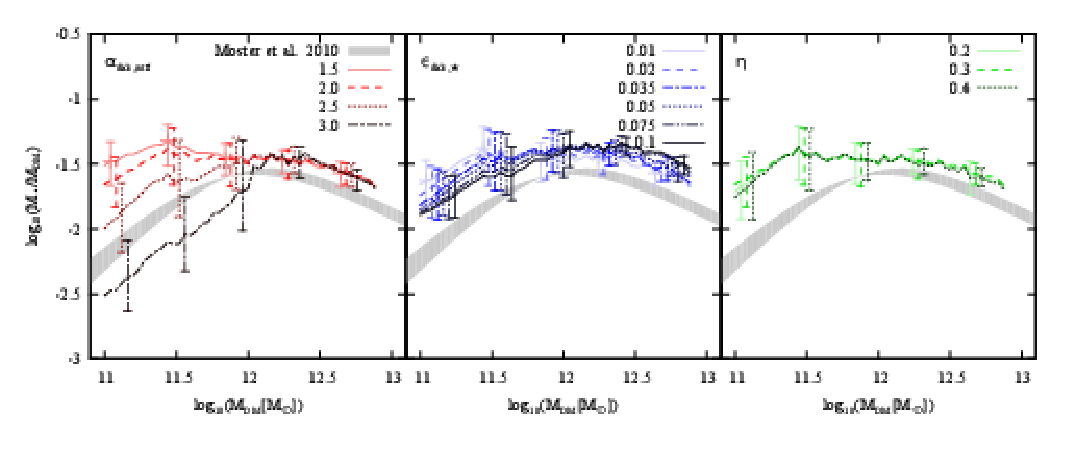
\includegraphics[scale=0.45,angle=0]{figures/runs/run-v1-13-multiplot-star-frac.eps}
%  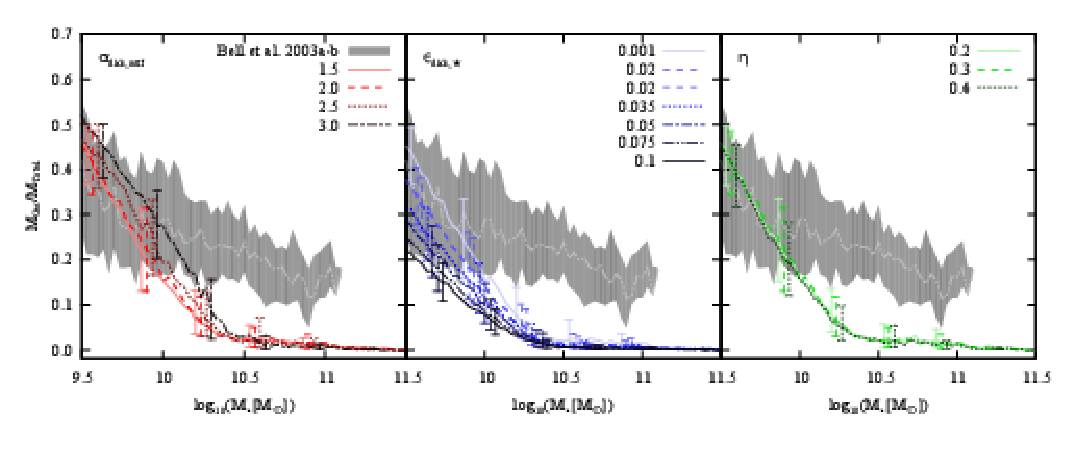
\includegraphics[scale=0.45,angle=0]{figures/runs/run-v1-13-multiplot-gas.eps}
%  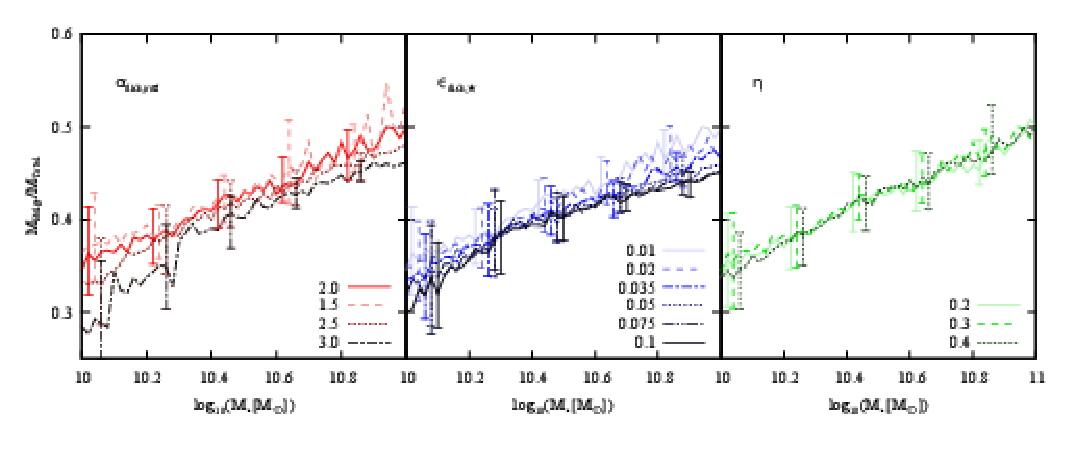
\includegraphics[scale=0.45,angle=0]{figures/runs/run-v1-13-multiplot-bulge.eps}
%\caption{...}
%\label{fig:runs}
%\end{figure}

%One might ask that in general the model parameters that are well
%suited to fit the observations of the LG galaxies are not necessarily
%the ones that are required to describe the general statistical
%properties of the galaxy population. To explore the answer to this
%question wee explore now the behaviour of different galaxy properties
%in our halo samples and compare the results against observations.

%Figure \ref{fig:runs} shows a summary of the runs shown in
%table \label{tab:runs} and his impact on variations on the parameters
%that characterise the galaxies in our definition: Stellar mass - halo
%mass fraction as a function of the stellar mass, gas mass to total
%ratio and bulge mass to total as a function of stellar mass. In
%general we see that in the halo mass regime explored in this work, the
%parameters that most affect the distributions are $\alpha_{outflow}$
%and $\epsilon_{\star}$. Nevertheless it is intriguing that in the case
%of $\alpha_{outflow}$, the value that best fits the results reported
%in the literature (Moster \etal 2010) for the general trend in the
%stellar-halo mass relation is $\alpha_{outflow} \sim 2.5-2.7$, but the
%value of $\alpha_{outflow} \sim 3$ clearly deviates from the expected
%at the low mass end. Nevertheless at the region of halo masses pf the
%order of $10^{12}$\hMsun it works quite well. The difference of the
%curves at lower halo masses should be due to ..... blah blah
%bla... (answer this point!).

%The same stellar mass-halo mass relation is seen to be not so strongly
%affected -in general- by variations on $\epsilon_{\star}$.  it
%can be seen that different values of $\epsilon_{\star}$ produce
%different stellar mass- halo mass relations, there are not really
%drastically different, conversely to what is observed with
%$\alpha_{outflow}$. For the specific case of the $\epsilon_{\star}$,
%again the value of $\epsilon_{\star}=0.01$ produces the relations more
%strongly deviated at the low mass end of the relation, close to the
%halo mass we are interested in $10^{12}$\hMsun, this value provides
%an acceptable match to the observations.

%Finally, as it can be seen in the figure variations on the final end
%of the material after merger (bulge or disk) does not really affect
%the stellar mass-halo mass relation in a noticeable manner. We can
%however observe that in general the stellar mass-halo mass relation we
%produce (even with the reference parameter values) is in general
%relatively high.

%Not so nice results are obtained for the gas to total mass ratio or
%the bulge to total mass ratio as a function of stellar mass. In
%general the scatter on the data is high enough to fit with almost all
%models on that mass regime below $10^{10.5}$\Msun. In general we see
%again that $\epsilon_{\star}$ and $\alpha_{outflow}$ parameter are the
%ones that induce noticeable differences in the mean value for the
%relations. Large values of $\alpha_{outflow}$ produce slightly more
%gas rich galaxies and simultaneously low mass bulges, while low
%$\epsilon_{\star}$ values produce galaxies with slightly more mass in
%gas and simultaneously larger bulge mass. Variations on the final
%fate of the material after merger, bulge or disk, again produce no
%major difference on the relations for the models. Despite the
%differences observed in the different runs with different model
%parameters, all results are equally compatible with observations in
%the stellar mass regime below $10^{10}$\Msun, although lower values
%of $\epsilon_{\star}$ produce mean quantities closer to observations.

%After this exercise we see that in general the value parameters we
%obtain as those that maximise the probability of a galaxy to be a
%milky way are also well suited to describe statistical the observables
%and might represent a valid region in the volume of parameter space
%reproducing the properties of the galaxy distribution, implying that
%no fictitious assumption must be made to maximise the number of
%LG-like galaxies.

\subsection{The LG candidates}


\begin{figure*}
  \includegraphics[scale=0.55,angle=270]{figures/hist_GasFrac_MW.ps}
  \includegraphics[scale=0.55,angle=270]{figures/hist_GasFrac_M31.ps}
\caption{Mean gas mass fraction, Bulge mass and total stellar mass of
  realisations of the MW and M31 as a function of the values of the
  parameters $\epsilon_{\star}$ and $\alpha_{outflow}$. Only points
  falling in the ranges of values associated with the property of each
  galaxy are shown. Squares show the data for MW while triangles show
  the data for M31 while the grey scale indicates the different values
  of the property.}
\label{fig:runCands}
\end{figure*}

Now we focus our attention on the candidates to MW and M31 galaxy in
our constrained simulations and study how the properties of these
galaxies change under variations of the model parameters. From the
constrained simulations we took the merger trees of these two
candidates to MW and M31 and ran our models several times variating
smoothly the values of the parameters $\epsilon_{\star}$ and
$\alpha_{out}$ and check how the galaxy properties change under such
variations. In order to account for the variance on the results, for
each galaxy defined by the couple of values
($\epsilon_{\star}$,$\alpha_{out}$), we ran 100 realisations for each
pair of values of the parameters. From that set we compute the median
value of the galaxy properties that are presented in Figure
\ref{fig:runCands}.

In Figure \ref{fig:runCands} we show the different galaxy properties:
gas-to-total mass fraction, stellar-to-total mass fraction and
bulge-to-total mass fraction all as a function of the values of the
parameters $\epsilon_{\star}$ and $\alpha_{out}$. In that figure each
line of plots is associated to the different realisations (10909,
16953 or 2710), since we have three different realisations providing
three pairs of candidates.

Not all points in the plane are shown. In that figure we only show the
points that fall inside the region of tolerance of the observational
constrains imposed in table \ref{tab:lg-observations}. Analysing this
figure would lead us to conclude which are the best values of the
parameters ($\epsilon_{\star}$, $\alpha_{out}$) one can use to
reproduce consistently the properties of the LG galaxies, or
conversely, which are the values of the parameters that characterise
the properties of the LG galaxies.

Ideally, the set of parameters ($\epsilon_{\star}$, $\alpha_{out}$)
that better describe the observations of the LG galaxies given the
constraints on the three candidates would be that resulting from the
intersection of the different data sets for the different
properties. That is, the values of the parameters ($\epsilon_{\star}$,
$\alpha_{out}$) that are able to reproduce simultaneously the three
observables for each candidate. These regions are shown in figure
\ref{fig:runCands} for the MW galaxy. In that figure we can clearly
see that depending on the realisation of the candidate there are
different regions in the ($\epsilon_{\star}$, $\alpha_{out}$) plane
that satisfy the observational constraint. We can also see that for a
given candidate the different properties can be reproduced differently
by different values of the parameters. Is in this way that for example
for the candidate 10909 almost all the plane in ($\epsilon_{\star}$,
$\alpha_{out}$) produces results that are consistent with the
observations of $M_*/M_{tot}$, while almost none of these points in
the same region of the plane produce results consistent with the
observations of $M_{bulge}/M_{tot}$ and only a reduced region of these
parameters is allowed by the constrain of the observations of
$M_{gas}/M_{tot}$. A similar behaviour can be seen for the candidates
in the other two boxes.

Analysing in detail, for a given candidate, only a very small portion
of the plane corresponding to the regions enclosed by the lines, are
those that correspond to regions where there is agreement for the
values of the parameters that reproduce the three observed constraints
of the MW galaxy. No much agreement (in a point by point basis)
between the different candidates is found.  However, what can be seen
is a clear trend on the values that favour the observations among the
three candidates. Specifically, almost all values of
$\epsilon_{\star}$ show to be able to reproduce the observed mass
fractions. On the other hand, not all values of $\alpha_{out}$ seem to
fit the constraint. Notice that values of $\alpha_{out}$ between 2.5
and 2.85 seems to favour the observables for all three candidates, in
agreement with the results shown in section \ref{sec:Probabilities}.

The scenario is quite more different for M31. As in can be seen in
Figure \ref{fig:runCands} (bottom), there is no intersection between
the regions on the plane ($\epsilon_{\star}$, $\alpha_{out}$) that for
a given candidate fits the observational constraints. Also, although
in agreement with what is found for MW almost all values of
$\epsilon_{\star}$ can satisfy the constraint, it is not as clear that
large values of $\alpha_{out}$ do so, not at least with the clarity is
can be seen for MW. Note also that in particular, $M_*/M_{tot}$ is not
well reproduced, in contrast to what is observed for MW and that in
general the fraction of area in the plane $M_*/M_{tot}$ is not well
reproduced, in contrast to what is observed for the MW. Finally one
can see that the fraction of area in the plane ($\epsilon_{\star}$,
$\alpha_{out}$) that is well described by the models is smaller. This
may imply two possibilities: One, that the parameter describing both
galaxies are very much different, or second, that as it was mentioned
in the previous section, it is very difficult to fit simultaneously
the observable properties of the galaxies in the local group, and it
may be even more evident for M31.


%%%%%%%%%%%%%%%%%%%%%%%%%%%%%%%%%%%%%%%%%%%%%%%%%%%%%%%%%%%%%%%%%%%%%%%
%%%%%%%%%%%%%%%%%%%%%%%%%%%%%%%%%%%%%%%%%%%%%%%%%%%%%%%%%%%%%%%%%%%%%%%
%%%%%%%%%%%%%%%%%%%%%%%%%%%%%%%%%%%%%%%%%%%%%%%%%%%%%%%%%%%%%%%%%%%%%%%


\section{Summary and discussion}

We have used numerical simulations of galaxy formation to estimate the
fraction of LG-like galaxies through the definition of a distance
measure in a N-dimensional parameter space in a sample of around 27000
model galaxies. The outcome of this initiative can be summarised as:

1) Through the more stringent distance measure defined in
eq. \ref{eq:distance} the fraction of galaxies similar to MW and M31
is zero when one tries to fit simultaneously all observables used to
define the LG galaxies.

2) Relaxing the form of the distance measure, and computing the
distance in a parameter-by-parameter basis one can find that there are
objects that fulfil the individual observational constraints, but
that these objects that satisfy one or two parameters do not satisfy
the others.

We have found however that in general all values of the parameter
$\epsilon_{\star}$ may be in agreement with observational constraints,
while larger values of $\alpha_{out}$ favour an increase in the
frequency of LG-like objects.

The simulations used in this work are constrained simulations of the
local Universe, and they have been ran in a way that a portion of the
simulation volume should reproduce the large scale environment of the
local group, as well as the small scale conditions to include a
candidate to host a Local Group. Using this constraint we have ran
several realisations of MW and M31 variating the model parameters
($\epsilon_{\star}$ and $\alpha_{out}$) in order to find the region of
this reduced parameter space that best reproduces the observations. In
agreement with the findings of the first part of the paper, we found
that the probability of reproducing simultaneously several properties
of the LG galaxies is very low.  Again we found that almost all values
of $\epsilon_{\star}$ are in agreement with the observational
constraints, while for MW values of $\alpha_{out}$ between 2.5 and
2.85 produce results that are in kind of agreement with the
observations. For M31 the volume of parameter space sampled by the
models is smaller, indicating that reproducing its properties is
somehow more difficult than for MW, or that the range of physical
parameters explaining the properties of both galaxies does not
overlap evenly.

Considering the size of the sample, and the nature of the constraints
(in the observations and in the simulations), a major conclusion out
of this work is that the major galaxies in the Local Group are not
that common.

In table \ref{tab:simulations} we have shown a larger plan of
simulations that it was discussed in the results. Variations on the
mass ratio $\eta$ defining the nature of the mergers does not change
the distributions of distance measures, that is, the galaxy population
does not change (relative to LG galaxies) under variations of the mass
threshold that defines the nature of the mergers, and therefore does
not affect the fraction of LG-like galaxies in our simulations. Moving
the material resulting from a merger to the bulge instead of the disk
also show not to influence noticeably the final population of
galaxies.  It seems to be related to the quiet mass accretion history
of the LG galaxies. As it has been shown in Forero-Romero \etal 2011,
the MAH of LG haloes is quiet. They also show that in general its MAH
does not bias from the general population of haloes in the same mass
range. That the galaxy population nor the fraction of LG-like galaxies
does not change much under variation of these parameters, is just a
consequence of the uniformity on the distribution of MAH's in our
simulations.

Note that in the first part of this work we do not constrain
explicitly the mass of the dark matter haloes. The mass range we are
using to study the fraction of LG-like galaxies is broad, $10^{11}$ to
$10^{13}$\hMsun, way much broader than any dark matter halo mass
estimated for the galaxies in the Local Group. We use such a broad
mass range just to allow a comparison with a larger halo and therefore
galaxy population and to avoid the imposition of a biasing by the
range of dark matter halo masses. However, the constraint in the halo
mass comes in the distance measure through the maximum circular
velocity of the galaxy $V_{cmax}$, which depends directly on the dark
matter halo mass, but that is related to the observables, conversely
to mass.

Implications:

de Rossi etal?
Boylan-Kolchin?


\section*{Acknowledgements}

The authors wants to tanks to DAAD and Colciencias for the financial
support through the bilateral collaboration PPP-PROCOL. Project
XXXXXXXX. J.C.M., J.F. and S.G. acknowledge the hospitality from
Universidad de Antioquia. S.S. and J.Z. acknowledge the hospitality
of the Leibniz Institut F\"{u}r Astrophysik Potsdam.

%%%%%%%%%%%%%%%%%%%%%%%%%%%%%%%%%%%%%%%%%%%%%%%%%%%%%%%%%%%%%%%%%%%%%%%
%%%%%%%%%%%%%%%%%%%%%%%%%%%%%%%%%%%%%%%%%%%%%%%%%%%%%%%%%%%%%%%%%%%%%%%


\begin{thebibliography}{99}


  
\end{thebibliography}


\bsp

\label{lastpage}

\end{document}


%\subsection{Verification tests}

%We show that the SAM and our tress and simulations reproduce the
%trends.

%A first test one should make is to see if our simulation, our post
%processing and merger tree constructions as well as the semi-analytic
%method are able to reproduce the basic observables on the distribution
%of galaxies.

%To do so we have just run GALACTICUS on out three boxes and compute
%the colour magnitude diagram and the I-band Tully-Fisher fisher
%relation.

%In Figure \ref{fig:T-F-diagram} we show the I-band Tully-Fisher
%relation. The data point are from Pizzano \etal (2007). The lines show
%the median value for the relation we obtain fro the runs R1, R2 and
%R3, where we have used the reference parameter values of GALACTICUS
%modifying only the redshift of reionization and the distribution of
%spin parameter. With the same simulations we have performed the
%comparison of the colour magnitude diagram obtained in our simulations
%with the data of the SDSS shown in Mu\~noz-Cuartas \& Mueller
%2012. The gray region shows the data from SDSS while the lines show
%the median values obtained from the model galaxies in our three boxes.
%As it can be seen, GALACTICUS can reproduce quite well obervables
%using our data, which give us confidence about the procedures
%implemented in the code and in the techniques we used to post analyse
%our N-body simulations.


%\begin{figure}
%  %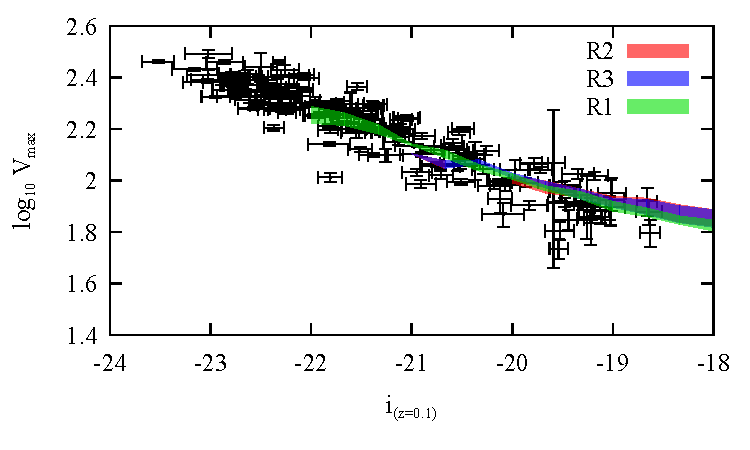
\includegraphics[scale=0.68, angle=0]{figures/tests/T_F-disk-velmax.pdf}
%\caption{ Tully-Fisher  relation. The magnitudes where calculated
%  without dust extinction and the parameters of the models can be seen
%  at Table \ref{tab:runs} as R1, R2 and R3. The error bars correspond
%  to the results of \citet{2007AJ....134..945P}.}
%\label{fig:T-F-diagram}
%\end{figure}


%\begin{figure}
%  %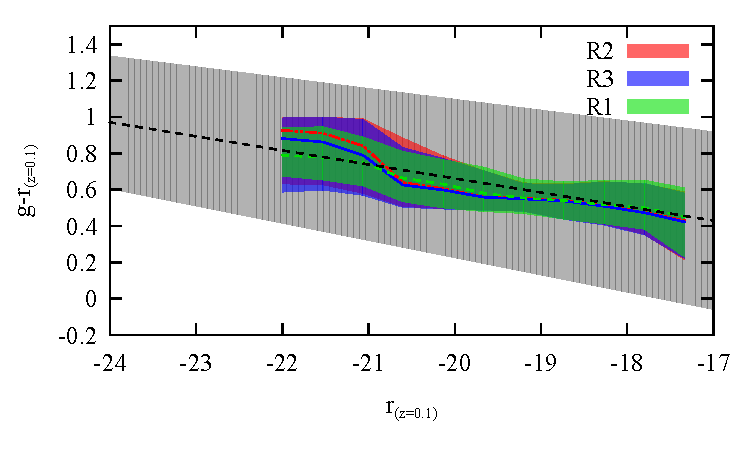
\includegraphics[scale=0.68,angle=0]{figures/tests/Color_Mag.pdf}
%\caption{ Colour magnitude relation. Magnitudes were calculated without
%  extinction. This is the reference simulation presented in table
%  \ref{tab:runs} as R1, R2 and R3. The shaded region correspond to a
%  scatter of $2\sigma$ from the work of
%  \citet{2012MNRAS.423.1583M}.\label{fig:CM-diagram}}
%\end{figure}
